\documentclass[9pt]{beamer}\usepackage[]{graphicx}\usepackage[]{color}
%% maxwidth is the original width if it is less than linewidth
%% otherwise use linewidth (to make sure the graphics do not exceed the margin)
\makeatletter
\def\maxwidth{ %
  \ifdim\Gin@nat@width>\linewidth
    \linewidth
  \else
    \Gin@nat@width
  \fi
}
\makeatother

\definecolor{fgcolor}{rgb}{0.345, 0.345, 0.345}
\newcommand{\hlnum}[1]{\textcolor[rgb]{0.686,0.059,0.569}{#1}}%
\newcommand{\hlstr}[1]{\textcolor[rgb]{0.192,0.494,0.8}{#1}}%
\newcommand{\hlcom}[1]{\textcolor[rgb]{0.678,0.584,0.686}{\textit{#1}}}%
\newcommand{\hlopt}[1]{\textcolor[rgb]{0,0,0}{#1}}%
\newcommand{\hlstd}[1]{\textcolor[rgb]{0.345,0.345,0.345}{#1}}%
\newcommand{\hlkwa}[1]{\textcolor[rgb]{0.161,0.373,0.58}{\textbf{#1}}}%
\newcommand{\hlkwb}[1]{\textcolor[rgb]{0.69,0.353,0.396}{#1}}%
\newcommand{\hlkwc}[1]{\textcolor[rgb]{0.333,0.667,0.333}{#1}}%
\newcommand{\hlkwd}[1]{\textcolor[rgb]{0.737,0.353,0.396}{\textbf{#1}}}%
\let\hlipl\hlkwb

\usepackage{framed}
\makeatletter
\newenvironment{kframe}{%
 \def\at@end@of@kframe{}%
 \ifinner\ifhmode%
  \def\at@end@of@kframe{\end{minipage}}%
  \begin{minipage}{\columnwidth}%
 \fi\fi%
 \def\FrameCommand##1{\hskip\@totalleftmargin \hskip-\fboxsep
 \colorbox{shadecolor}{##1}\hskip-\fboxsep
     % There is no \\@totalrightmargin, so:
     \hskip-\linewidth \hskip-\@totalleftmargin \hskip\columnwidth}%
 \MakeFramed {\advance\hsize-\width
   \@totalleftmargin\z@ \linewidth\hsize
   \@setminipage}}%
 {\par\unskip\endMakeFramed%
 \at@end@of@kframe}
\makeatother

\definecolor{shadecolor}{rgb}{.97, .97, .97}
\definecolor{messagecolor}{rgb}{0, 0, 0}
\definecolor{warningcolor}{rgb}{1, 0, 1}
\definecolor{errorcolor}{rgb}{1, 0, 0}
\newenvironment{knitrout}{}{} % an empty environment to be redefined in TeX

\usepackage{alltt}

\usepackage{framed}
\usepackage{alltt}
\usepackage{amsmath}
\usepackage{mathtools}
\usepackage{graphicx, color}
\usepackage{natbib}
\usepackage{hyperref}
\usepackage{mathptmx}
\usepackage{beamerthemesplit}
\usepackage{lipsum}

\graphicspath{{../report/figs/}}

\setbeamersize{text margin left=5pt,text margin right=5pt}
\parskip 3mm

\definecolor{firebrick}{RGB}{178,34,34}
\useinnertheme{circles,rounded}
\usecolortheme[named=firebrick]{structure}
\useoutertheme{smoothtree}
\setbeamertemplate{footline}[frame number]

\title{Bayesian inference for covariance matrix}
\author{Ignacio Alvarez-Castro}
\institute[IESTA]{ Center of Statistical Research (IESTA) \\ Universidad de la República, Uruguay.}
\date{2nd - 6th July 2018. University of St Andrews. \\ 
International Statistical Ecology Conference.}
\IfFileExists{upquote.sty}{\usepackage{upquote}}{}
\begin{document}
 \frame{\titlepage}
 
 \section{Introduction}
\AtBeginSection[] { 
  \begin{frame}[plain]  
    \tableofcontents[currentsection] 
  \end{frame} 
  \addtocounter{framenumber}{-1} 
} 


	\frame{
		\frametitle{Introduction}
Covariance matrix estimation		
\begin{itemize} \itemsep2em
\item  Multivariate normal sampling models 
\item random-intercept, random-slope models 
\begin{eqnarray}
\nonumber y_{ij} &=& \beta_{0j} + \beta_{1j} x_{ij} + \beta_{2j}z_{ij} + \epsilon_{ij} \\
\nonumber  \begin{pmatrix} \beta_{0j} \\ \beta_{1j} \\ \beta_{2j} \end{pmatrix} &\sim&  N \left( \begin{pmatrix} \mu_{0} \\ \mu_{1} \\ \mu_{2} \end{pmatrix} , \Sigma \right) , \;\;\; \epsilon_{ij} \sim N(0, \sigma^2) 
%\nonumber \epsilon &\sim& N(0, \sigma^2) 
\end{eqnarray}

\item \cite{ovaskainen2017make} includes covariance matrix priors for comunity data hierarchical models
\end{itemize}
}

\subsection{Motivation example}
\begin{frame}
\frametitle{Bird counts on Superior forests}
 The Natural Resources Research Institute (University of Minnesota Duluth) carry out monitoring program for study regional population trends of forest birds.
%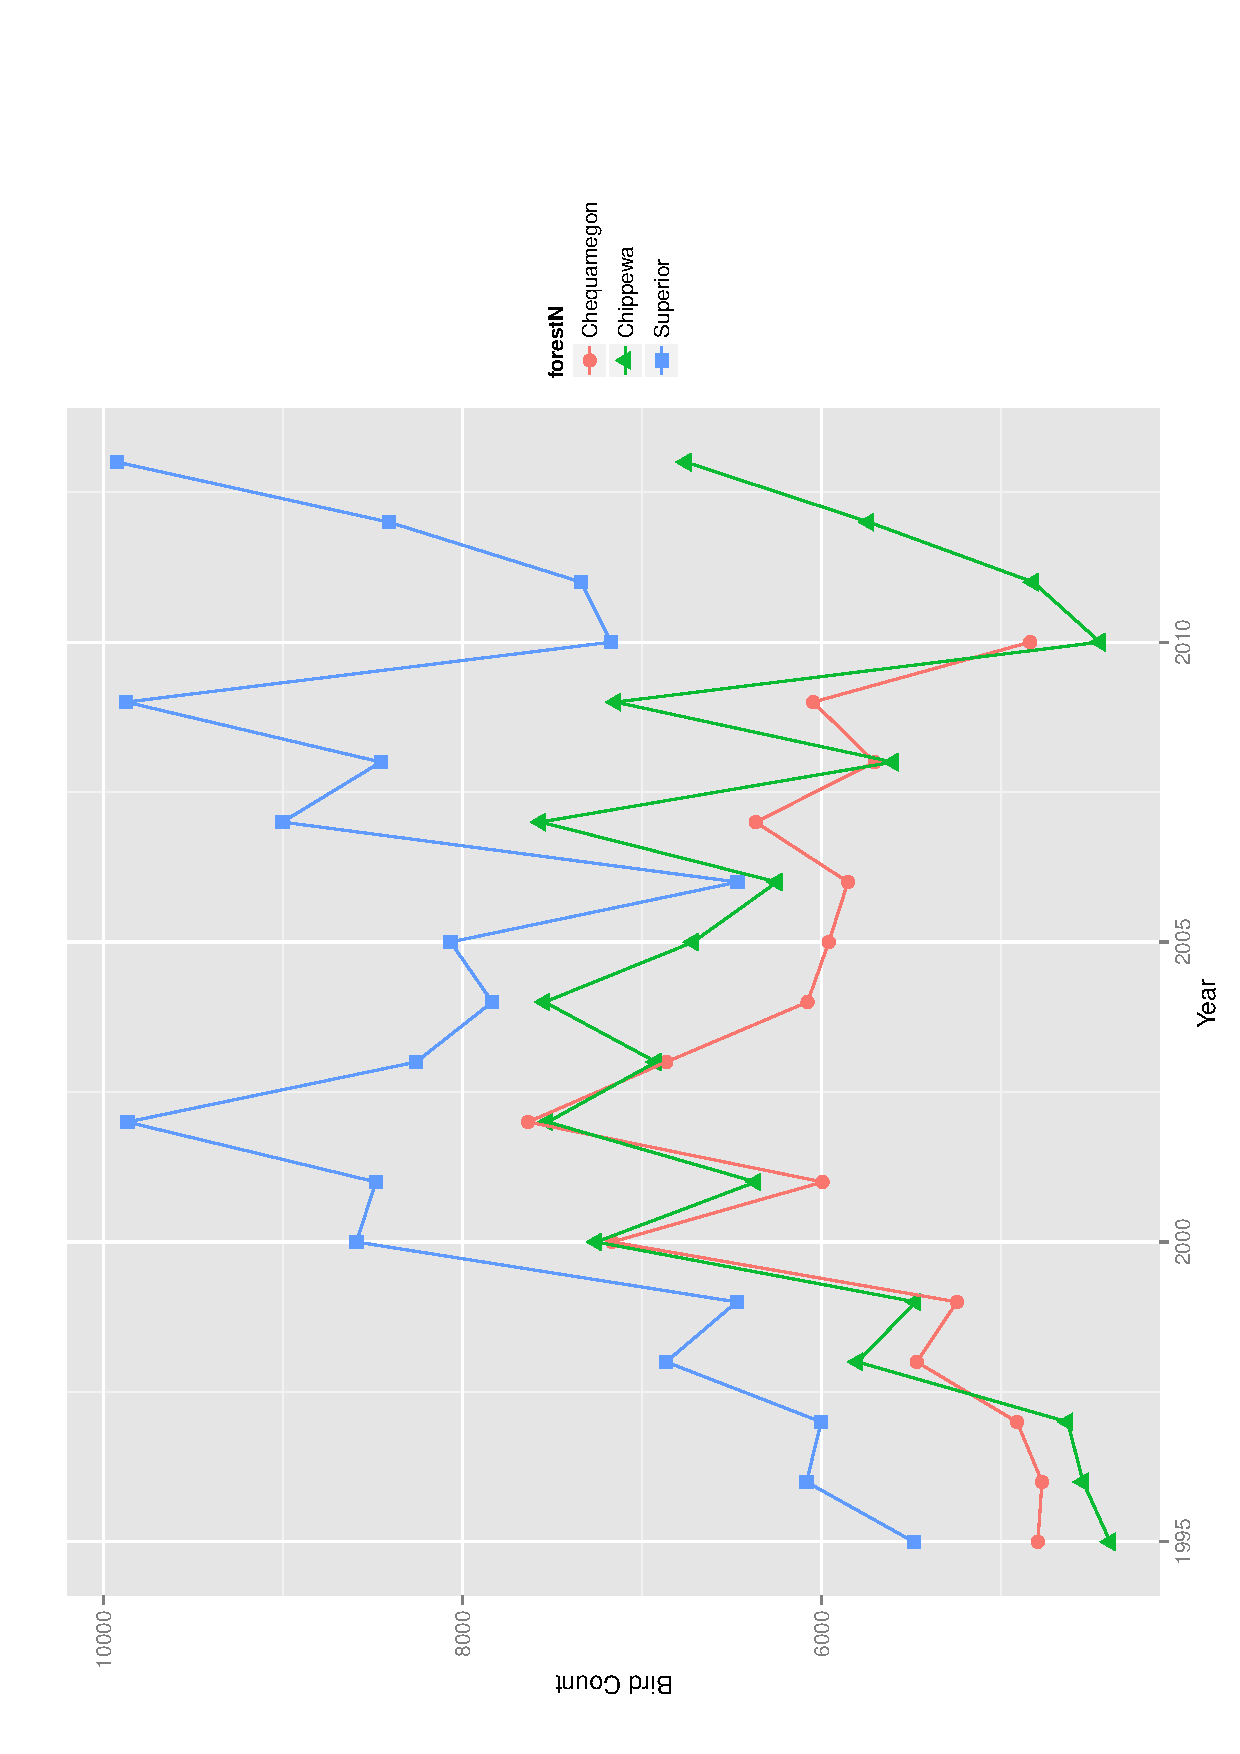
\includegraphics[width=\textwidth, height = 7cm ]{rawtrend}
\vspace{.5cm}

Want to study population trend over time
\[
E(y_{st})  = \beta_{0s} + \beta_{1s} t + \beta_{2t}t^2
\]

\begin{columns}
\begin{column}{4cm}
Point count for :
\begin{itemize}
  \item 19 years (1995 - 2013)
  \item 3 forest
  \item 73 bird species
\end{itemize}
\end{column}
\begin{column}{5cm}
Response $y_{st}$
\begin{itemize}
  \item Total count in logs
  \item Average count accros sites
  \item Total count
\end{itemize}

\end{column}
\end{columns}

\end{frame}

\begin{frame}
\frametitle{Quadratic trend model}
  \begin{columns}[T] % the "c" option specifies center vertical alignment
  \column{.5\textwidth} % column designated by a command
Separate model for each species:
\begin{itemize}
  \item $y_{st}$: bird count for spacies $s$ in year $t$.
  \item OLS regression model 
\end{itemize}

\[
y_{st}  \sim  N(\beta_{0s} + \beta_{1s} t + \beta_{2t}t^2, \sigma^2)
\]

\vspace{.5cm}
Correlation among coefficient estimates
\begin{description}
  \item[Total in logs] Corr$(\hat\beta_{1s}, \hat\beta_{2s}) = -.77$
  \item[Average] Corr$(\hat\beta_{1s}, \hat\beta_{2s}) = -.94$
  \item[Total] Corr$(\hat\beta_{1s}, \hat\beta_{2s}) = -.88$
\end{description}

  \column{.5\textwidth}
    \includegraphics[scale=.3]{ols_regs}
  \end{columns}

\end{frame}

\begin{frame}
\frametitle{Quadratic trend model}

Hierarchical linear model with $IW$ prior. 

\[\begin{array}{cl}
y_{st}  & \sim  N(\beta_{0s} + \beta_{1s} t + \beta_{2t}t^2, \sigma^2) \\
& \\
\begin{pmatrix} \beta_{0j} \\ \beta_{1j} \\ \beta_{2j} \end{pmatrix} & \sim  N \left( \begin{pmatrix} 0 \\ 0 \\ 0 \end{pmatrix} , \Sigma \right) \\
& \\
\Sigma & \sim  IW(d+1, I)
\end{array}
\]

Correlation among coefficient
\[ \rho = \Sigma_{23}/\sqrt{\Sigma_{22}\Sigma_{33}} \]

\end{frame}

\begin{frame}
\frametitle{Quadratic trend model}

Hierarchical linear model with $IW$ prior. Posterior $p(\rho | y)$

\begin{center}
\includegraphics[trim= 0cm 2cm 0cm 3cm, clip, scale=.7]{reg_3modIW}
\end{center}

\end{frame}

%============

\section{Multivariate normal model } 
\begin{frame}
\frametitle{Multivariate normal model }

\cite{Alvarez2014} compare alternative priors for $\Sigma$ in this for multivariate normal data.
\[ Y_i \sim N_d(0, \Sigma) \]

Alternative $\Sigma$ priors
\begin{itemize}
\item Inverse Wishart: $IW(\nu, \Lambda)$:  $p(\Sigma) \propto  |\Sigma|^{-(\nu+ d +1)/2 } e^{-\frac{1}{2} tr( \Lambda \Sigma^{-1}) }$

\item Scaled Inverse Wishart 
\item Hierarchical inverse Wishart
\item Separation strategy 
\end{itemize}

Asses prior inpact on posterior inference:
\begin{itemize}
\item using simulations
\item with the bird count data set (not shown)
\end{itemize}
\end{frame}






% \begin{frame}
% \frametitle{ Samples from prior }
% 
% \begin{figure}[htbp]
% \begin{center}
%  \includegraphics[scale=.3]{prior_sis2} 
% \end{center}
% \end{figure}
% 
% Positive relationship among $\sigma_1$ and $\sigma_2$, also large $|\rho_{12}|$ values appear when the two variances are high.
% \end{frame}



\begin{frame}
\frametitle{Impact on posterior inference}
Inference for $\rho_{12}$
	\begin{columns}
	 \begin{column}{7cm}
		 \begin{figure}[hbtp]
		   \includegraphics[scale=.4]{fig_rho_d2} 
		\end{figure}
	\end{column}
	\begin{column}{4cm}
	When standard deviation is small, $\sigma=0.01$ or $\sigma=0.1$ the IW prior heavily shrinks the posterior correlation towards 0 even if the true correlation is close to 1. 
	\end{column}
	\end{columns}
\end{frame}

\begin{frame}
\frametitle{Impact on posterior inference}
Inference for $\sigma_1$
	\begin{columns}
	 \begin{column}{7cm}
\begin{figure}[htbp]
   \includegraphics[scale=.4]{fig_s1_d2} 
%   \caption{Scatter-plot of posterior mean for $\sigma_1$  against correlation true standard deviation.}
\end{figure}
	\end{column}
	\begin{column}{4cm}
$IW$ prior overestimate the standard deviation when its true value is very low
 	\end{column}
	\end{columns}
\end{frame}

% \section{Separation strategy in linear model}
% \begin{frame}
% \frametitle{Separation strategy in linear model}
%   \begin{columns}[T] % the "c" option specifies center vertical alignment
%   \column{.5\textwidth} % column designated by a command
% 
% 
% \[\begin{array}{cl}
% y_{st}  & \sim  N(\beta_{0s} + \beta_{1s} t + \beta_{2t}t^2, \sigma^2) \\
% & \\
% \begin{pmatrix} \beta_{0s} \\ \beta_{1s} \\ \beta_{2s} \end{pmatrix} & \sim  N \left( \begin{pmatrix} 0 \\ 0 \\ 0 \end{pmatrix} , \Sigma \right) \\
% & \\
% \Sigma & = \mbox{diag}(\lambda)\; \Omega\; \mbox{diag}(\lambda) \\
% & \\
% \lambda_k & \sim Ca^+(0, 1) \\ 
% & \\
% \Omega & \sim LKJ(3) 
% \end{array}
% \]
% 
%   \column{.5\textwidth}
%   \pause
%   Posterior $p(\rho| y)$ 
%     %\includegraphics[scale=.3]{reg_rho_den}
%   \end{columns}
% \end{frame}



\section{Discussion}

\begin{frame}
\frametitle{Discussion}
Prior choice (based on multivariate normal data results)
\begin{enumerate} \itemsep1em
\item Separation strategy  gives modeling flexibility and good inferences properties. \citep{barnard2000}
\item In Gibbs base samplers a prior which maintain conjugacy might be preferable (scaled inverse Wishart or hierarchical inverse Wishart) 
\item If we are constraint to use $IW$, we may recommend to scale the data first.
\end{enumerate}  
\vspace{.5cm}

Future steps
\begin{description} \itemsep1em
\item[Different Model] Hierarchical linear model context. 

\item[Different Priors] Use $LKJ$ prior for the correlation matrix. 

Use other distributions for $IW$ parameters $\nu$ and $\Lambda$.
\end{description}
\end{frame}


\begin{frame}
\frametitle{References}
  \bibliographystyle{../report/asa}      
\small{  \bibliography{../report/library} }
\end{frame}


\end{document}
